\documentclass{article}

\usepackage{graphicx} 
\usepackage{subfigure}
\usepackage{paralist}

\usepackage{hyperref}

\usepackage{url}
\usepackage{booktabs}

\usepackage[usenames,dvipsnames]{xcolor}
\usepackage{tikz}
\usetikzlibrary{positioning, calc}

\usepackage[draft,nomargin,footnote]{fixme}

\graphicspath{{figs/}}

\usepackage{xspace}
\newcommand{\eg}{\textit{e.g.}\xspace}
\newcommand{\etal}{\textit{et al.}\xspace}
\newcommand{\ie}{\textit{i.e.}\xspace}
\newcommand{\etc}{\textit{etc.}\xspace}
\newcommand{\vs}{\textit{vs.}\xspace}

\title{Learning by Teaching a Robot: the Case of Handwriting}

\author{S\'everin Lemaignan, Alexis Jacq, Fernando Garcia, Ana Paiva, Pierre
Dillenbourg \\ CHILI Lab, \'Ecole Polytechnique F\'ed\'erale de Lausanne}


\begin{document}
\maketitle

\begin{abstract}
    TDB
\end{abstract}


%%%%%%%%%%%%%%%%%%%%%%%%%%%%%%%%%%%%%%%%%%%%%%%%%%%%%%%%%%%%%%%%%%%%%%%%%%%%%%%%%%%
%%%%%%%%%%%%%%%%%%%%%%%%%%%%%%%%%%%%%%%%%%%%%%%%%%%%%%%%%%%%%%%%%%%%%%%%%%%%%%%%%%%
%%%%%%%%%%%%%%%%%%%%%%%%%%%%%%%%%%%%%%%%%%%%%%%%%%%%%%%%%%%%%%%%%%%%%%%%%%%%%%%%%%%
\section{A different paradigm for educative robots}

Henry is five and an half, and has been diagnosed with visuo-constructive
deficits. He is under the care of an occupational therapist, and tries to improve
his inability to draw letters in a consistent manner. Diego is six and struggles
at school with his poor handwriting and even poorer self-confidence.

While Henry is lively and always quick at shifting his attention from one
activity to another, Diego is shy and poised. Two very different children,
facing however the same difficulty to write in a legible manner.


\begin{figure}
    \centering
    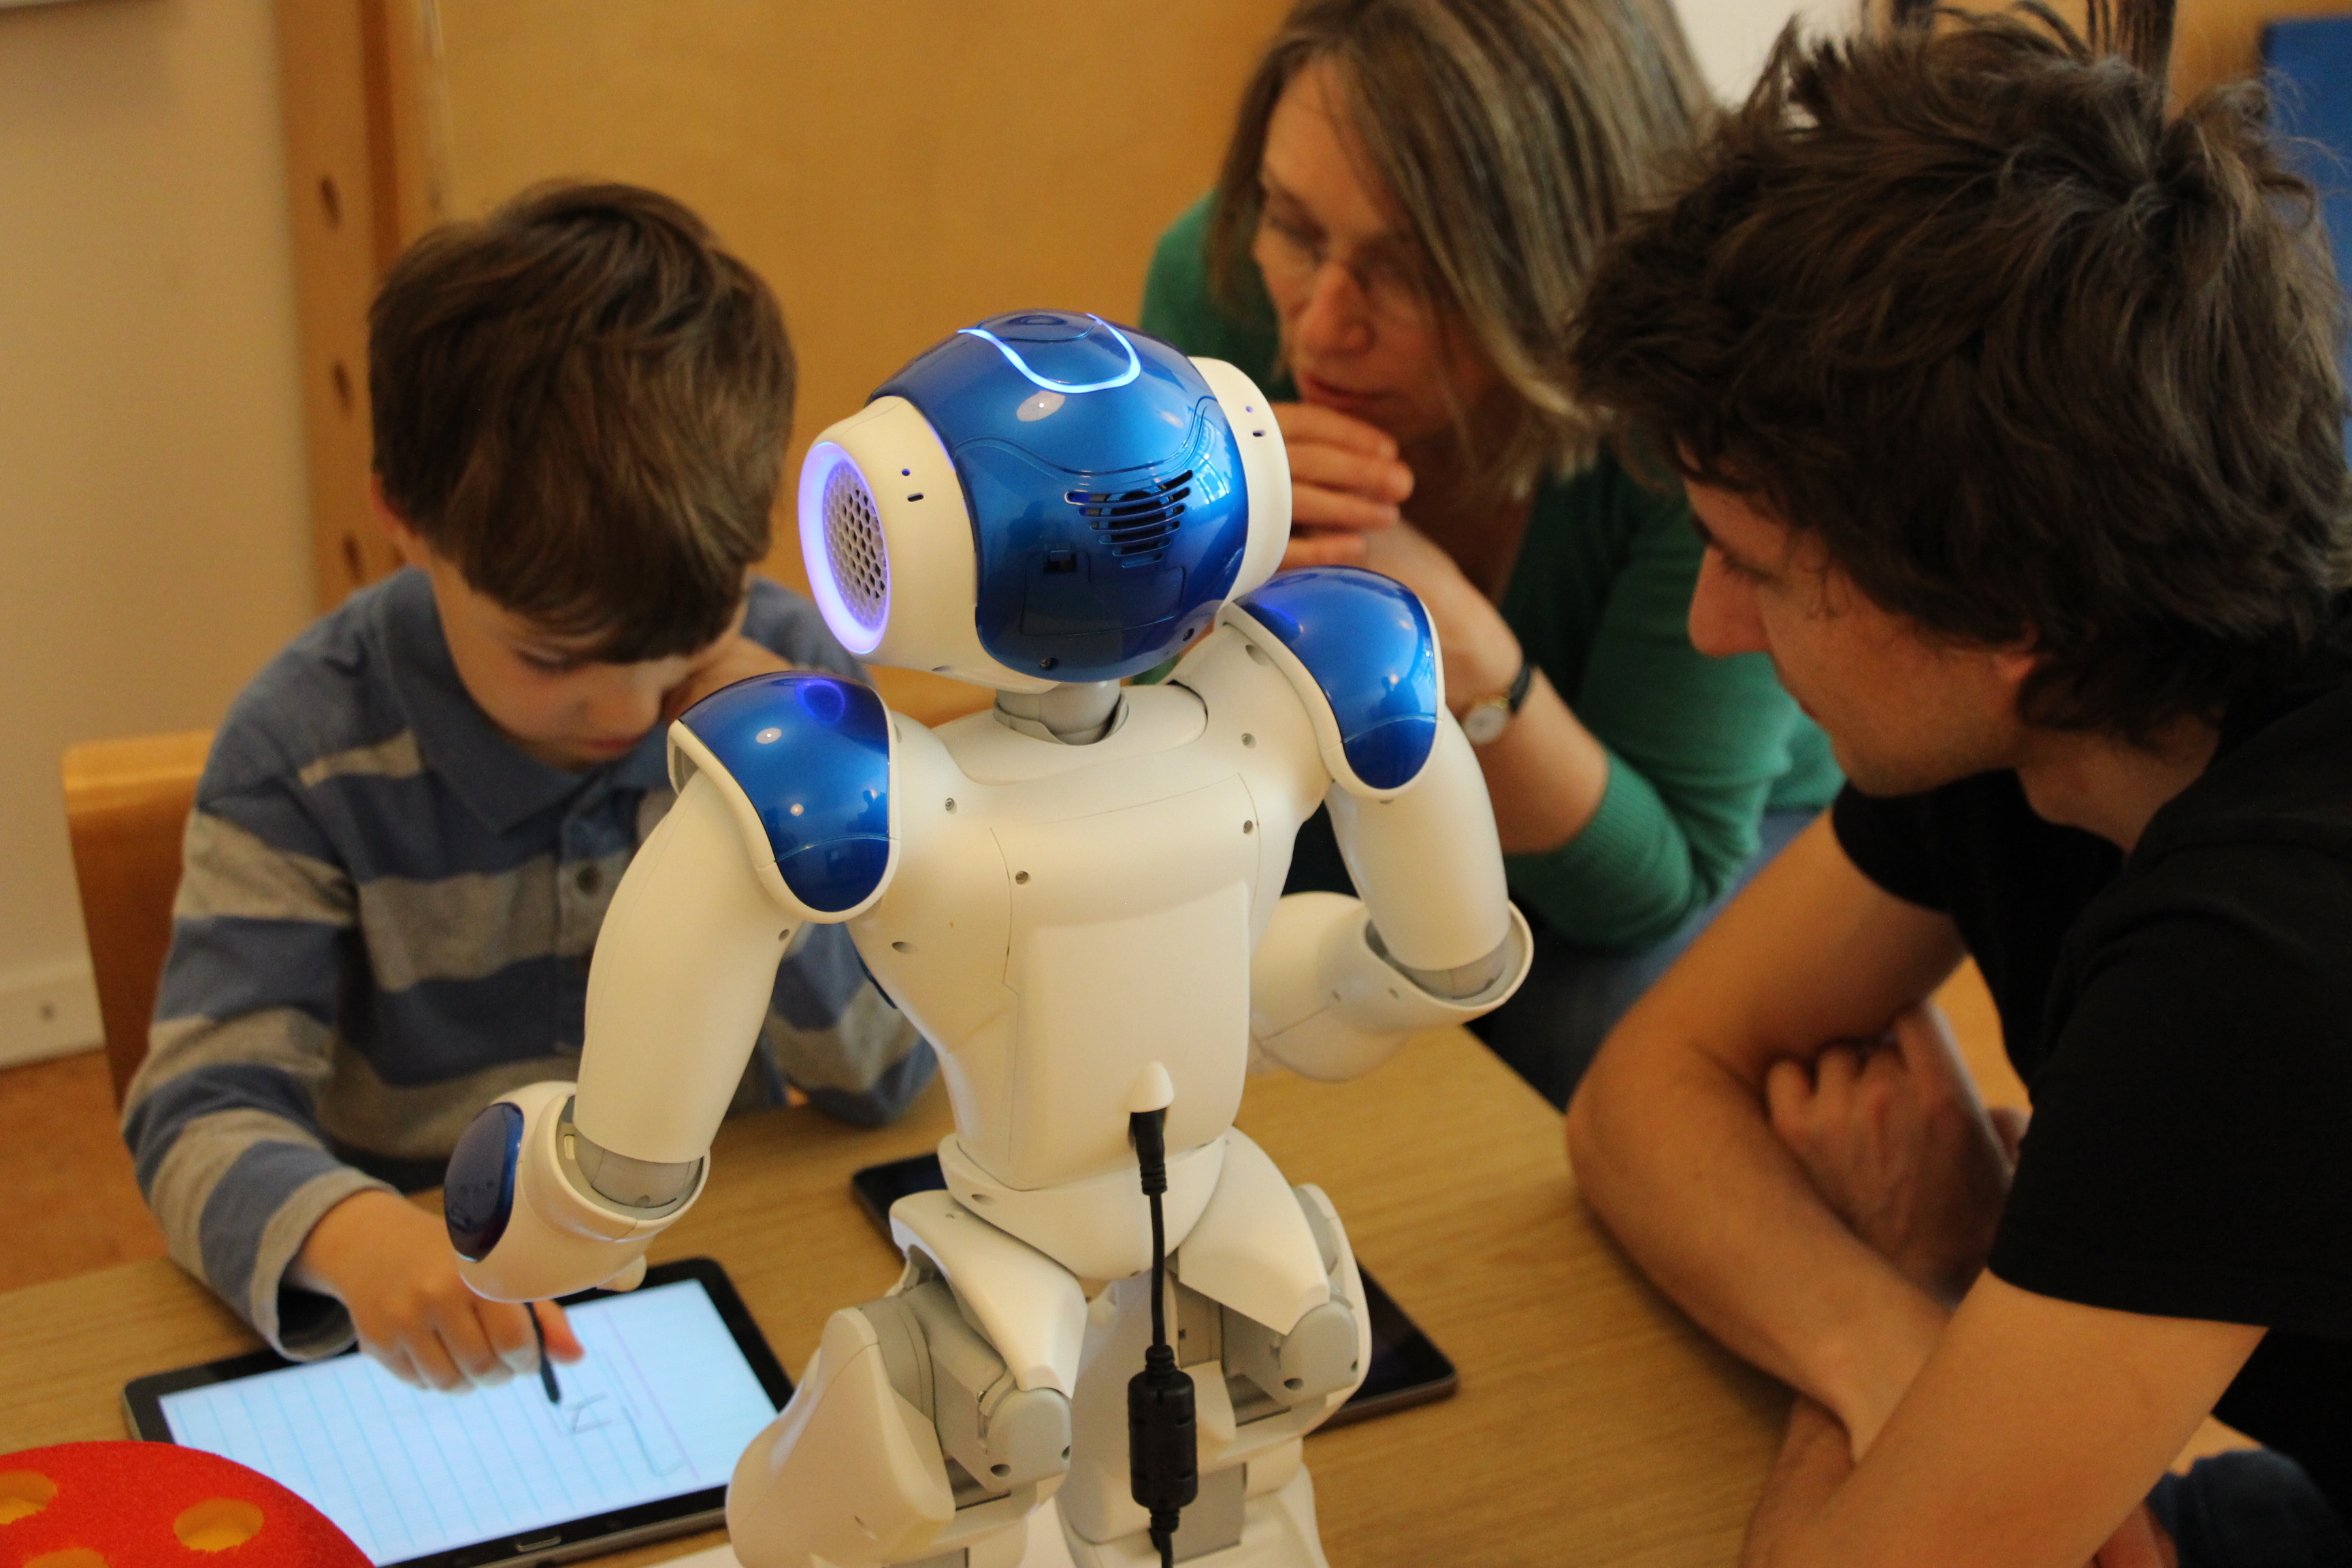
\includegraphics[width=0.9\linewidth]{henry}
    \caption{Henry teaching Nao how to write numbers, with the help of an
    occupational therapist.}
    \label{fig:henry}
\end{figure}

Remediations for handwriting difficulties

\subsection{Learning by Teaching}

The \emph{learning by teaching} paradigm, which engages the target student in
the act of teaching another, has been shown to produce motivational,
meta-cognitive, and educational benefits in a range of disciplines~\cite{Rohrbeck2003}. 
To our best knowledge, the application of the paradigm to
handwriting intervention remains, however, unexplored. One reason for this may
due to the requirement of an appropriately unskilled peer for the target child
to tutor, as this may present a logistical constraint if the target child is the
lowest performer in their class.  In some cases, it may be appropriate for a
peer or teacher to simulate a na\"ive learner for the target child to teach.
For handwriting, where one's skill level is visually evident, however, this
acting is likely to be eventually detected. As such, there is motivation for the
use of a teachable agent which can be configured for a variety of skill levels,
and for which children do not have preconceptions about its handwriting ability.

Robots have been used as teachers or social partners to promote children's
learning in a range of contexts, most commonly related to language
skills~\cite{han2010robot}, and less often to physical skills (such as
calligraphy~\cite{Matsui2013}).  Looking at the converse (humans \emph{teaching}
robots), Werfel notes in~\cite{Werfel2014} that most of the work focuses on the
robot's benefits (in terms of language~\cite{Saunders2010} or
physical~\cite{Mulling2013} skills, for example) rather than the learning
experienced by the human tutor themselves.  Our work concentrates on this latter
aspect: by demonstrating handwriting to a robot, we aim at improving the
\emph{child's} performance. Note that our work must be distinguished from
``learning from demonstration'' approaches to robots learning physical skills,
as the agent we present is only simulating fine motor skills for interaction
purposes.

A robotic learning agent which employs the learning by teaching paradigm has
previously been developed by Tanaka and Matsuzoe~\cite{Tanaka2012}. In their
system, children learn vocabulary by teaching the {\sc nao} robot to act out
verbs. The robot is tele-operated and mimics the actions that the children teach
it, but with no long-term memory or learning algorithm in place.  Our project
significantly extends this line of work in two ways. First, by investigating the
context of children's acquisition of a challenging physical skill (handwriting),
and second by proposing a robotic partner which is fully autonomous in its
learning.


\subsection{Teaching beyond ICT}

This research departs from the traditional approaches to educative robotics
(\fixme{cite reviews})

Also notable, the robot is not used in the usual context of robotics or computer
education, but instead in an activity -- handwriting -- which requires fine
physical skills. In such activities, the embodied nature of the robot is
appropriate as in interventions where motor mimicry is elicited
\cite{Berninger1997} the arm motion for instance is, \emph{by itself}, part of
the teaching. Furthermore, when facing a child with school difficulties, robots
can play the role of a na\"ive learner which neither adults nor peers -- because
of the social effects it would induce -- can convincingly play. Along these
lines, we hope to see more research on non-STEM educational applications of
robotics.

Beyond handwriting, we believe that this work provides a novel perspective on
the role for robots in the field of education. \emph{Learning by teaching} is a
powerful paradigm because of not only its pedagogical efficacy, but its
potential to positively impact the child's motivation and self-esteem. We hope that 
this article shows that this is a very relevant context of use for robots. Indeed,
when facing a child with school difficulties, robots can play the role of a na\"ive 
learner which neither adults nor peers -- because of the social effects it would 
induce -- can convincingly play.


%%%%%%%%%%%%%%%%%%%%%%%%%%%%%%%%%%%%%%%%%%%%%%%%%%%%%%%%%%%%%%%%%%%%%%%%%%%%%%%%%%%
%%%%%%%%%%%%%%%%%%%%%%%%%%%%%%%%%%%%%%%%%%%%%%%%%%%%%%%%%%%%%%%%%%%%%%%%%%%%%%%%%%%
%%%%%%%%%%%%%%%%%%%%%%%%%%%%%%%%%%%%%%%%%%%%%%%%%%%%%%%%%%%%%%%%%%%%%%%%%%%%%%%%%%%
\section{Implementation of the Interaction}

Figure~\ref{experimental_setup} illustrates our general experimental setup: a
face-to-face child-robot interaction with an (autonomous) Aldebran's Nao robot.

A tactile tablet (with a custom application) is used for both the robot and the
child to write: during a typical round, the child requests the robot to write
something (a single letter, a number or a full word), and push the tablet
towards the robot, the robot writes on the tablet by gesturing the writing, but
\emph{without actually physically touching the tablet}), the child then pull
back the tablet, correct the robot's attempt by writing him/herself on top or
next to the robot's writing (see the picture in Figure~\ref{fig:diego}), and
``send'' his/her demonstration to the robot by pressing a small button on the
tablet. The robot ``learns'' from this demonstration and tries again.

Since the child is assumed to take on the role of the teacher, we had to ensure
he/she would be able to manage by him/herself the turn-taking and the overall
progression of the activity (moving to the next letter or word). In our design,
the turn-taking relies on the robot prompting for feedback once it is done with
its writing (simple sentences like ``What do you think?''), and pressing on a
small robot icon on the tablet once the child has finished correcting. In our
experiments, both were easy to grasp for children.


\begin{figure}
    \centering
    
\includegraphics[width=0.8\linewidth]{experimental_setup}
    \caption{Our experimental setup: face-to-face interaction with a Nao robot.
    The robot writes on the tactile tablet, the child then corrects the robot by
    directly overwriting its letters on the tablet, with a stylus directly. An adult
    (either a therapist or an experimenter, depending on the studies), remains next
    to the child to guide the work (prompting, turn taking, etc.). For some studies, a second tablet and an additional camera (dashed) are employed.}
    \label{experimental_setup}
\end{figure}

Implementing such a system raises several challenges: first, acquiring,
analyzing and learning from hand-written demonstration lays at the core of the
our approach and we developed several algorithms for the robot to generate
initial bad writing and to respond in an adequate manner, showing visible (but
not too quick) writing improvements.

Then, the actual implementation on the robot required the coordination of
several modules (from performing gestures and acquiring the user's input to
the high-level state machine), spread over several machines (the robot itself,
one laptop and up to four tactile tablets for certain studies we conducted). We
relied on ROS to ensure the synchronization and communication between these
modules.

Finally, the interaction itself, involving a robot, one or two children and, in
one study, an occupational therapist, also raised by itself several challenges.

We detail each of these points in the following sections.

%%%%%%%%%%%%%%%%%%%%%%%%%%%%%%%%%%%%%%%%%%%%%%%%%%%%%%%%%%%%%%%%%%%%%%%%%%%%%%%%%%%
\subsection{Algorithmic Approach}

\begin{figure}[thpb]
    \centering
    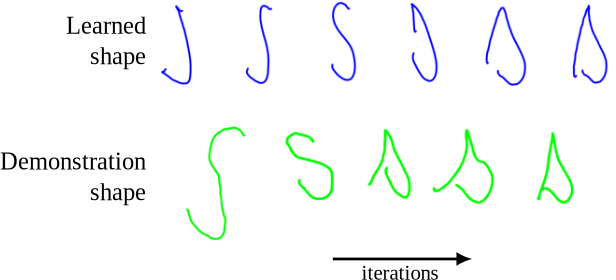
\includegraphics[width=0.6\columnwidth]{learningSdemo}
    \caption{\label{fig:demonstrationShapes2}Example of the learning algorithm
    responding (top) to user demonstration of shapes (bottom) for the letter `s'
    (demonstrations received from two 7-8 year-old children taking turns).}

\end{figure}


\subsubsection{Path Manipulation in the Letters' Eigenspace}

\begin{figure}[ht!]
    \centering
    \subfigure[Nine samples of the cursive ``h'', next to the reference]{
        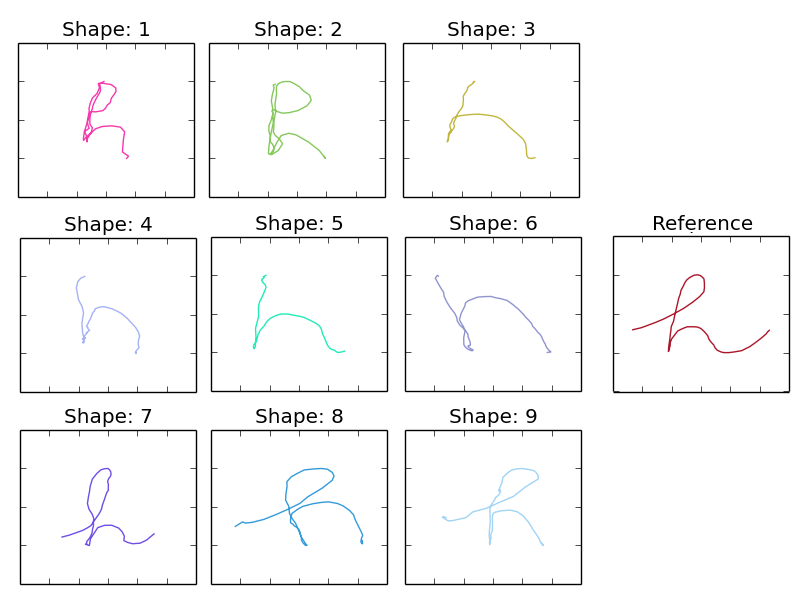
\includegraphics[height=6cm]{h}
    }
    \subfigure[Raw samples projected in the Eigenspace of the dataset]{
        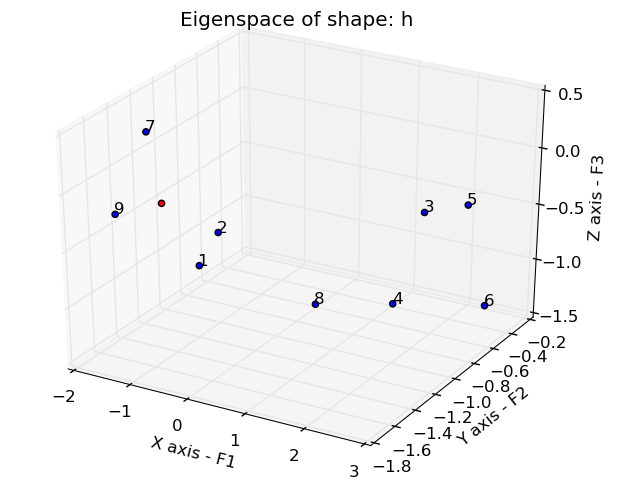
\includegraphics[height=4cm]{eigenspace-base}
    }
    \subfigure[Normalized samples, projected in the Eigenspace. The letters are
    clustered according to their styles.]{
        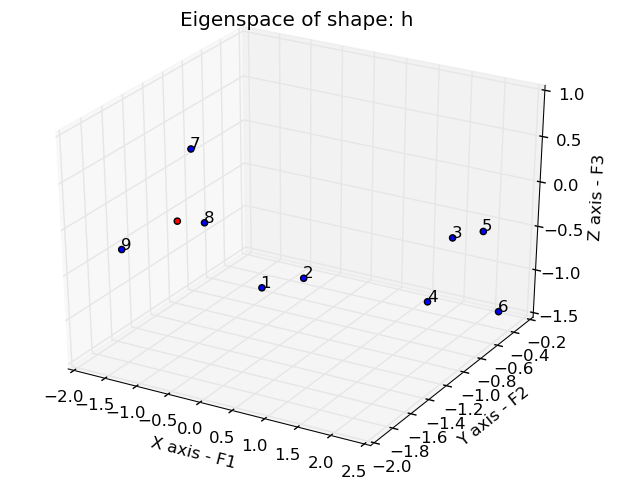
\includegraphics[height=4cm]{eigenspace-uniformization}
    }

    \caption{\small Projecting demonstrated letters onto the Eigenspace
    generated from the reference dataset effectively clusters the samples
according to their topological similarity.}
    \label{fig:stimuli}
\end{figure}


%%%%%%%%%%%%%%%%%%%%%%%%%%%%%%%%%%%%%%%%%%%%%%%%%%%%%%%%%%%%%%%%%%%%%%%%%%%%%%%%%%%
\subsection{Robotic Implementation}

In order to develop a teachable agent that is appropriate for engaging a child
in the learning by teaching paradigm, we have established capabilities for the
robot to engage in handwriting and interactive turn-taking.

The {\sc nao} V4 humanoid robot, which has been purposely designed by Aldebaran
Robotics to look approachable~\cite{Gouaillier2008}, is used for this work. It
is a commercially affordable biped robot, 58cm tall, with 25 degrees of freedom,
two cameras, speech capabilities and the ability to autonomously execute a range
of tasks.

Precise control over what the robot is writing is necessary in the proposed
application of a handwriting. Because of the limited fine motor skills possible
with such an affordable robot, in addition to the absence of force feedback and
other technical necessities, we have configured the {\sc nao} to use simulated
handwriting with a synchronised tablet to achieve this level of control. 

The development of the necessary components for embedding the handwriting
learning algorithm presented in Section \ref{sec:learningAlgorithm} in the
humanoid agent are presented in the sections which follow.

\subsubsection{Robot Trajectory Following Movements}

Using simulated handwriting provides an opportunity for the robot's writing to
appear smoother than would be achievable with a writing instrument. However, the
robot's motions must still sufficiently match the displayed trajectory in order
capture the engagement of the child participant in the action. Aldebaran's NaoQi
API is used for the inverse kinematics of the trajectory following. The Robot
Operating System (ROS)\footnote{The ROS stack for {\sc nao} is available at:
\url{http://wiki.ros.org/nao_robot}.} is used for integration of the {\sc nao}
with external reference frames, such as the tablet's location, using the $tf$
transformation library \cite{Foote2013}.

When using simulated handwriting, it is no longer necessary that the robot
engages in the typical style of handwriting of using a writing instrument at a
desk.  Having the robot point at a vertical writing surface to cause the
trajectory to appear (as in Figure \ref{fig:naoWriting}) has several advantages:

\begin{itemize}

    \item The working space of the robot increases, both in the technical sense
        and the interaction sense: someone can, in theory, show the tablet to
        the robot from across the room and have it still respond, without
        needing the tablet to be within arm's reach.

    \item Concerns about whether or not the child would start mimicking the
        robot's incorrect writing form (\eg pen grip) are mitigated. 

    \item Perhaps most significantly, the accuracy of the matching of the
        robot's motion with the trajectory displayed on the tablet is not as
        critical. This is because a pen tip would be expected to touch the
        tablet exactly at the trajectory point, while a fingertip may not.

\end{itemize}

\begin{figure}[thpb]
     \begin{center}
            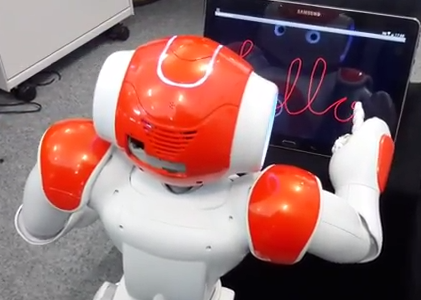
\includegraphics[width=0.7\linewidth]{naoWriting2.png}
    \end{center}
    \caption{A demonstration of the robot simulating the writing of a word with
    its finger. The motion of the robot is synchronised with the display of the
    tablet, communicating over ROS.}%

   \label{fig:naoWriting}
\end{figure}

We have therefore designed the system in such a way that the robot is simulating
handwriting by pointing at the tablet\footnote{Teachers interviewed for their
feedback on the system advised that children are asked to draw letters in
the air in a similar manner as part of their handwriting education. The
behaviour is hence not unfamiliar to children.}. As interacting with a
tablet with one's finger is not uncommon, this may aid the acceptance of the
writing style by users. 

Because motion planning is performed with respect to the hand of the robot,
rather than its fingertip, one or two of the orientation degrees of freedom of
the hand are fixed to keep the finger approximately perpendicular to the writing
surface, depending on the desired accuracy. The remaining free orientation(s),
coupled with the whole-body motion control available, allow for a sufficient
working space for writing on the entire tablet.


\begin{figure}[ht]
\centering

\resizebox{0.9\linewidth}{!}{%

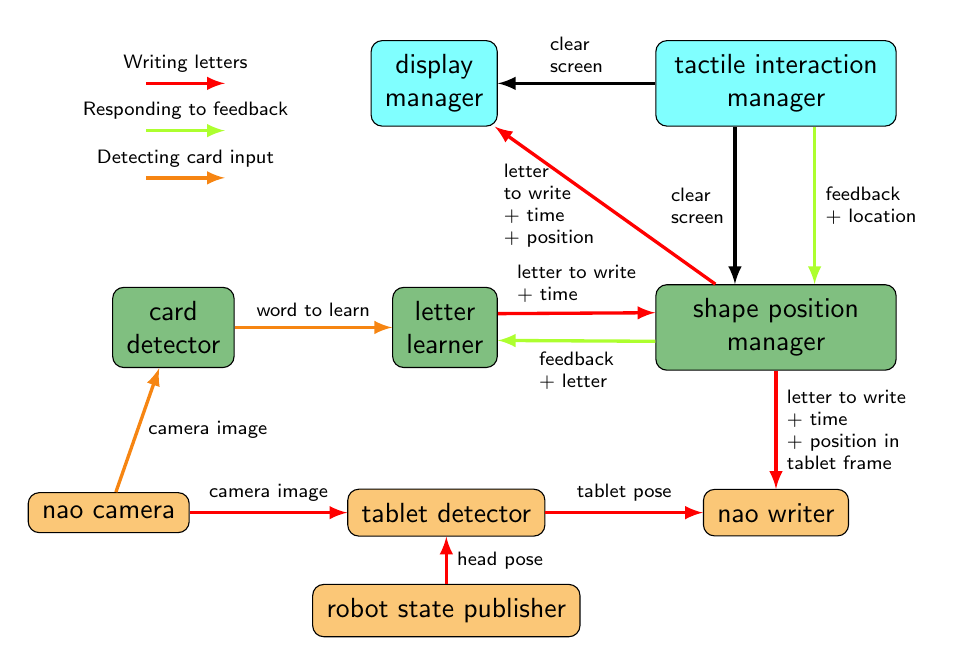
\begin{tikzpicture}[
    >=latex,
    node distance=2cm,
    every edge/.style={draw, very thick},
    redarrow/.style={fill=Red, draw=Red},
    greenarrow/.style={fill=GreenYellow, draw=GreenYellow},
    yellowarrow/.style={fill=BurntOrange, draw=BurntOrange},
    cmpt/.style={draw, align=center, rounded corners, inner sep=5pt, font=\sf, fill=black!20},
    label/.style={midway, align=left, font=\scriptsize\sf, fill=white, above,opacity=0,text opacity=1}]

    \node at (0,0)[cmpt, fill=Cyan!50, text width=2.7cm] (tactile) {tactile interaction \\ manager};
    \node[cmpt, fill=Cyan!50, left=of tactile] (display) {display \\ manager};
  
    \node [cmpt, fill=Green!50, below=of tactile, text width=2.7cm] (shape) {shape position \\ manager};
    \node [cmpt, fill=Green!50, left=of shape] (learner) {letter \\ learner};
    \node [cmpt, fill=Green!50, left=of learner] (card) {card \\ detector};

    \node [cmpt, fill=YellowOrange!50, below=1.5cm of shape] (writer) {nao writer};
    \node [cmpt, fill=YellowOrange!50, left=of writer] (tablet) {tablet detector};
    \node [cmpt, fill=YellowOrange!50, left=of tablet] (camera) {nao camera};
    \node [cmpt, fill=YellowOrange!50, below=0.6cm of tablet] (pose) {robot state publisher};

    %%% Relations between components
    \path (tactile) edge [->] node[label] {clear \\ screen} (display);

    \path ($(shape.north west)!0.33!(shape.north east)$) edge [<-] node[label,left] {clear \\ screen} ($(tactile.south west)!0.33!(tactile.south east)$);
    \path ($(shape.north west)!0.66!(shape.north east)$) edge [<-, greenarrow] node[label,right] {feedback \\ + location} ($(tactile.south west)!0.66!(tactile.south east)$);

    \path (shape) edge [->, redarrow] node[label, left, align=left] {letter \\to write \\ + time \\ + position} (display);
    \path (shape) edge [->,redarrow] node[label, right] {letter to write \\ + time \\ + position in\\tablet frame} (writer);

    \path ($(shape.north west)!0.66!(shape.south west)$) edge [->, greenarrow] node[label,below] {feedback \\ + letter} ($(learner.north east)!0.66!(learner.south east)$);
    \path ($(shape.north west)!0.33!(shape.south west)$) edge [<-, redarrow] node[label] {letter to write \\ + time} ($(learner.north east)!0.33!(learner.south east)$);

    \path (card) edge [->, yellowarrow] node[label] {word to learn} (learner);
    \path (camera) edge [->, yellowarrow] node[label, right] {camera image} (card);
    \path (camera) edge [->, redarrow] node[label] {camera image} (tablet);
    \path (tablet) edge [->, redarrow] node[label] {tablet pose} (writer);
    \path (pose) edge [->, redarrow] node[label, right] {head pose} (tablet);

    \path (-8, 0) edge [->, redarrow] node[label] {Writing letters} (-7, 0);
    \path (-8, -0.6) edge [->, greenarrow] node[label] {Responding to feedback} (-7, -0.6);
    \path (-8, -1.2) edge [->, yellowarrow] node[label] {Detecting card input} (-7, -1.2);
    
\end{tikzpicture}
}

\caption{Overview of the system. Components in the top row run on the tablet, 
those in the middle row on the central controller, and those in the bottom row 
on the robot.}

    \label{fig:archi}
\end{figure}



%%%%%%%%%%%%%%%%%%%%%%%%%%%%%%%%%%%%%%%%%%%%%%%%%%%%%%%%%%%%%%%%%%%%%%%%%%%%%%%%%%%
\subsection{Interaction Design}



%%%%%%%%%%%%%%%%%%%%%%%%%%%%%%%%%%%%%%%%%%%%%%%%%%%%%%%%%%%%%%%%%%%%%%%%%%%%%%%%%%%
%%%%%%%%%%%%%%%%%%%%%%%%%%%%%%%%%%%%%%%%%%%%%%%%%%%%%%%%%%%%%%%%%%%%%%%%%%%%%%%%%%%
%%%%%%%%%%%%%%%%%%%%%%%%%%%%%%%%%%%%%%%%%%%%%%%%%%%%%%%%%%%%%%%%%%%%%%%%%%%%%%%%%%%
\section{Field Studies}

To date, the presented system has been deployed and tested in three different
schools (totalling child-robot interactions with more than 70 children, aged 5
to 8) and we also conducted 2 case studies over several weeks.
Table~\ref{studies} gives an overview of these studies.

\begin{table}[ht!]
\centering
\caption{Field studies conducted within the project}
\label{studies}
\begin{tabular}{@{}lp{4.5cm}p{2.2cm}p{2.5cm}l@{}}
\toprule
{\bf Study}     & {\bf Type}                                    & {\bf Duration}              & {\bf Children \#}                     & {\bf Ages} \\ \midrule
{\it ISG 1}     & Unstructured group interaction at school      & 16 min/group               & 4 $\times$ 8 children                 & 6-7        \\
{\it Florimont} & Individual/Pair interaction at school         & 11 min/group               & 7 (individual) + 7 $\times$ 2 (pairs) & 7-8        \\
{\it Diego}     & Case-study, spanning over 4 weeks              & 1.5 hours $\times$ 4 weeks & 1                                     & 5          \\
{\it Haut-Lac}  & Pair (with turn-taking) interaction at school & 26 min/group                            & 7 $\times$ 2                          & 5-6        \\
{\it ISG 2}     & Individual interaction at school              & 18 min                            & 6                                     & 5-6        \\
{\it Henry}     & Case-study, spanning over 4 weeks              & 1h $\times$ 4 weeks        & 1                                     & 5          \\ \bottomrule
\end{tabular}
\end{table}

%%%%%%%%%%%%%%%%%%%%%%%%%%%%%%%%%%%%%%%%%%%%%%%%%%%%%%%%%%%%%%%%%%%%%%%%%%%%%%%%%%%
\subsection{Studies at School}

\begin{figure}
    \centering
    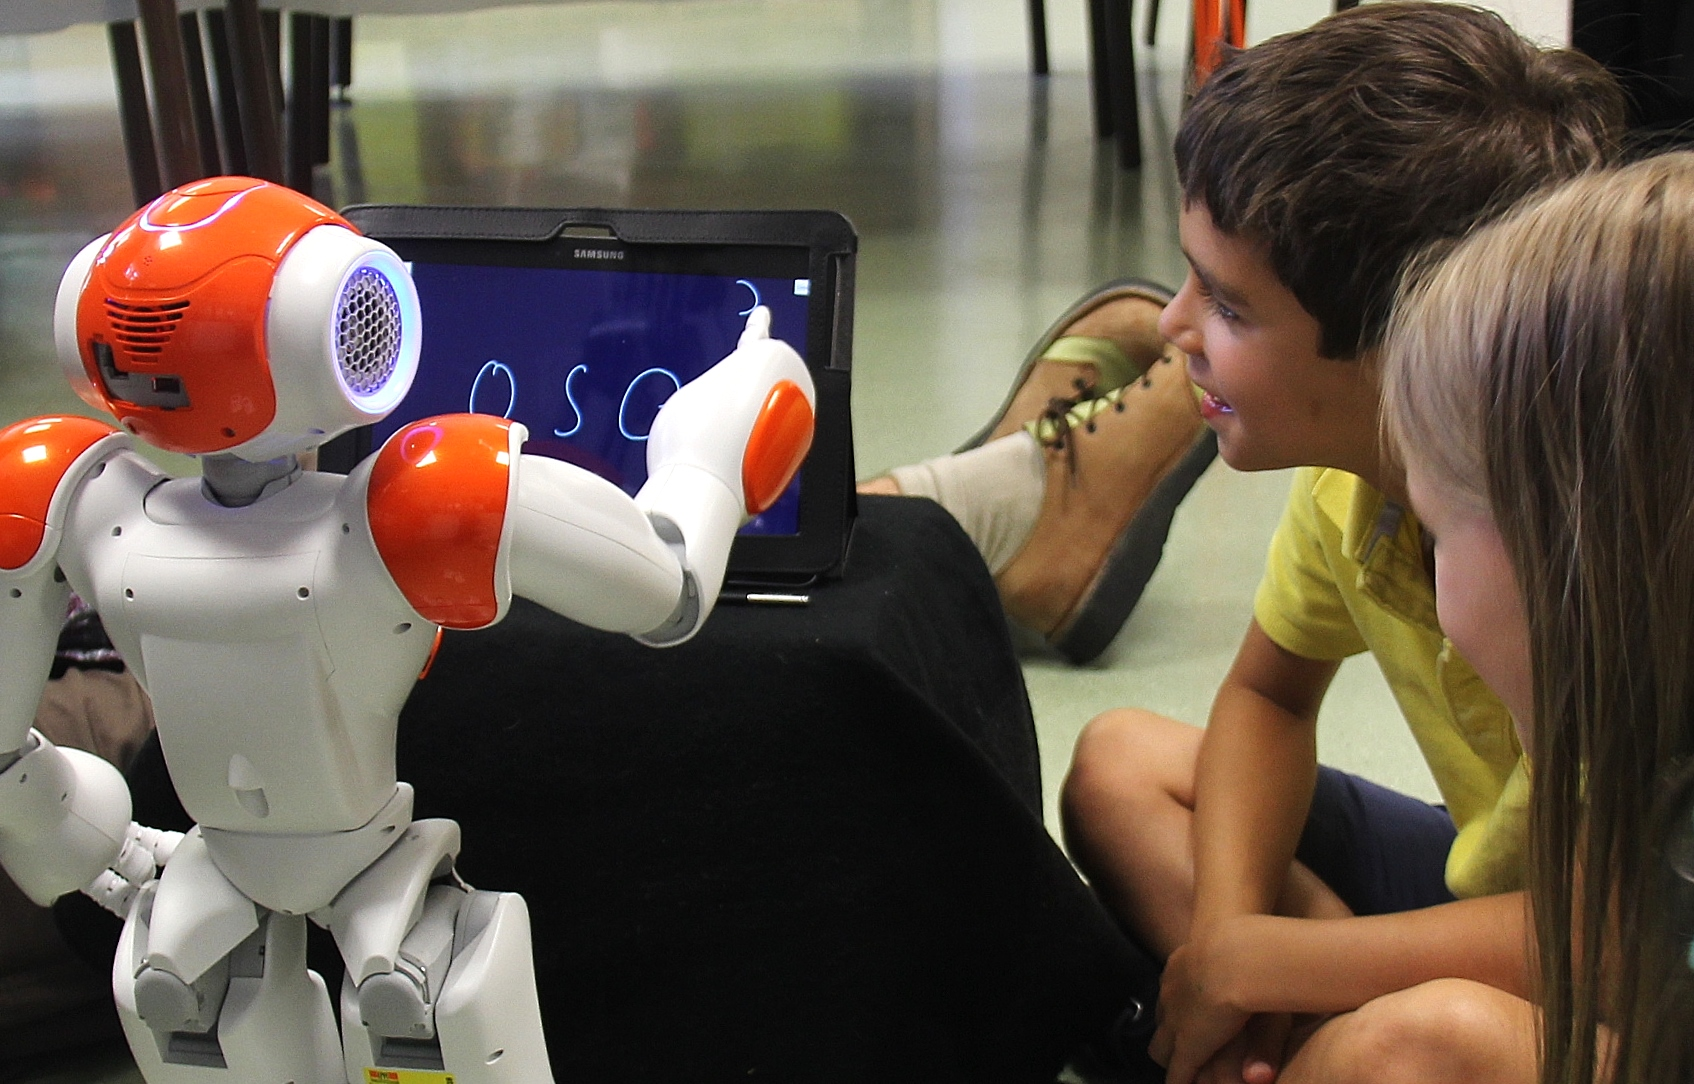
\includegraphics[height=3.9cm]{schools}
    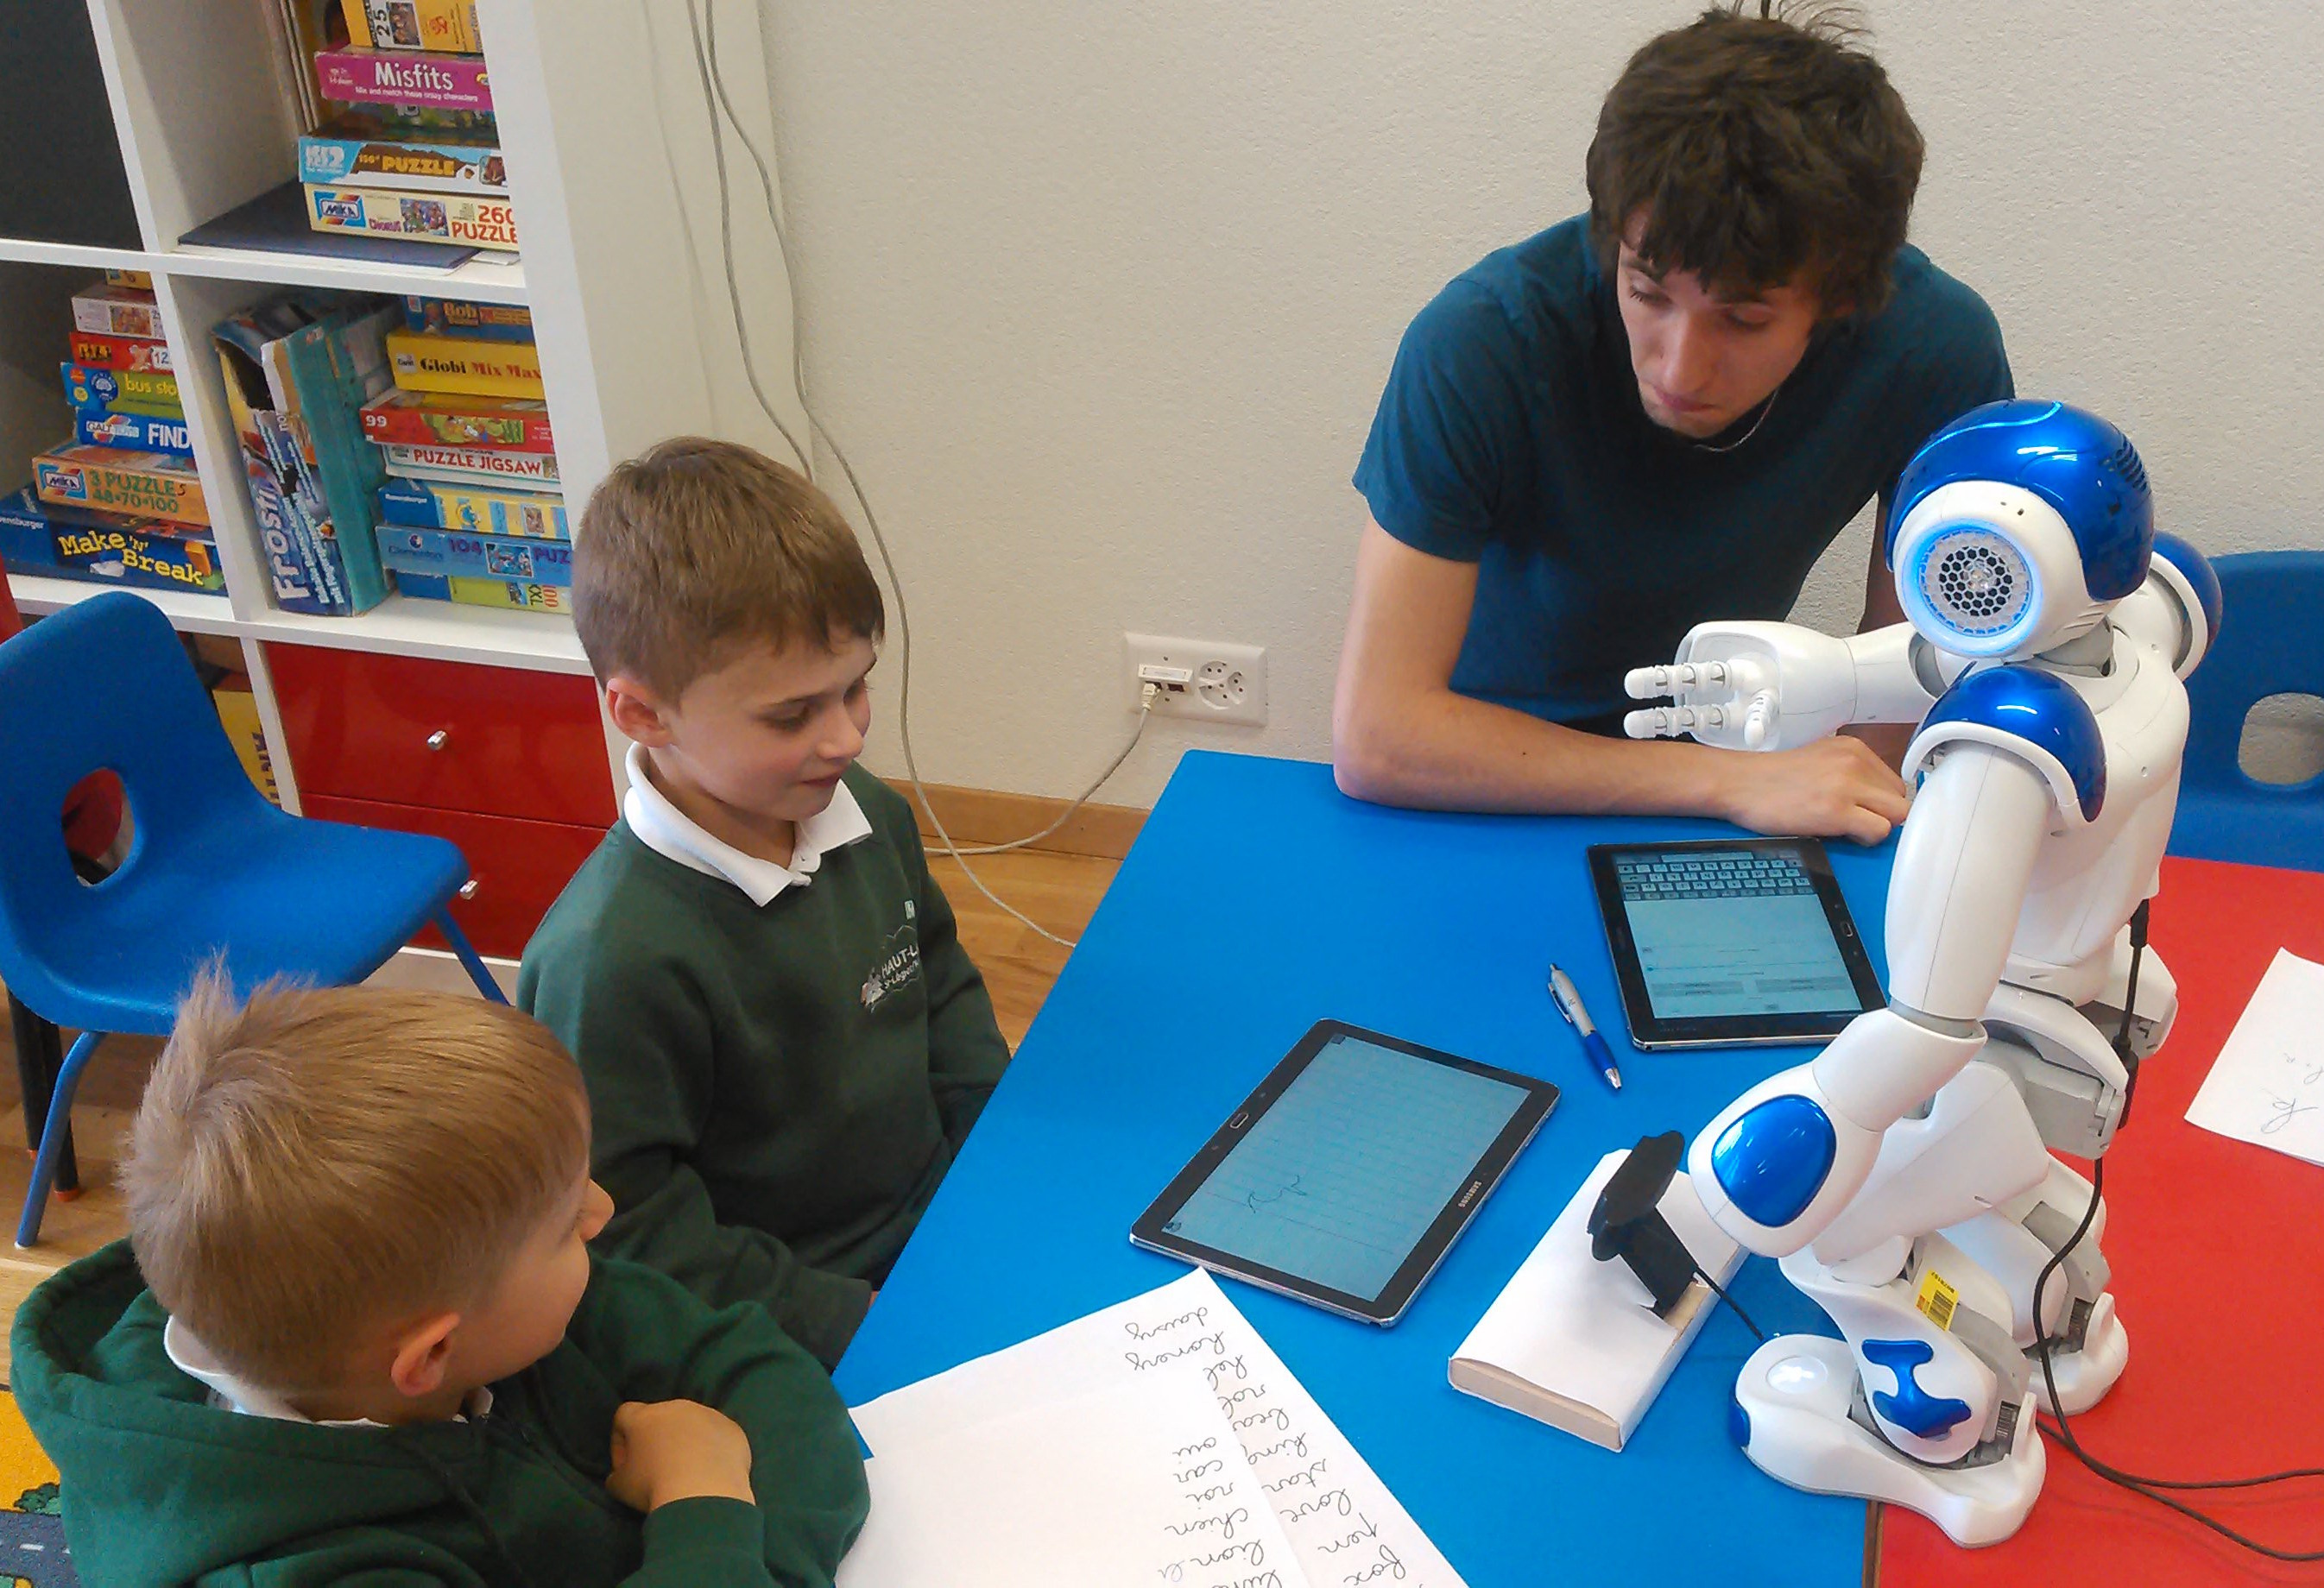
\includegraphics[height=3.9cm]{schools2}
    \caption{The first field studies were focused on technical validation, with
    above 70 pupils interacting with the robot over short periods (around 15
minutes), either alone or in small groups.}
    \label{fig:schools}
\end{figure}

%%%%%%%%%%%%%%%%%%%%%%%%%%%%%%%%%%%%%%%%%%%%%%%%%%%%%%%%%%%%%%%%%%%%%%%%%%%%%%%%%%%
\subsection{Case Study 1: Diego}

\subsubsection{Context, Study Design}

\begin{figure}
    \centering
    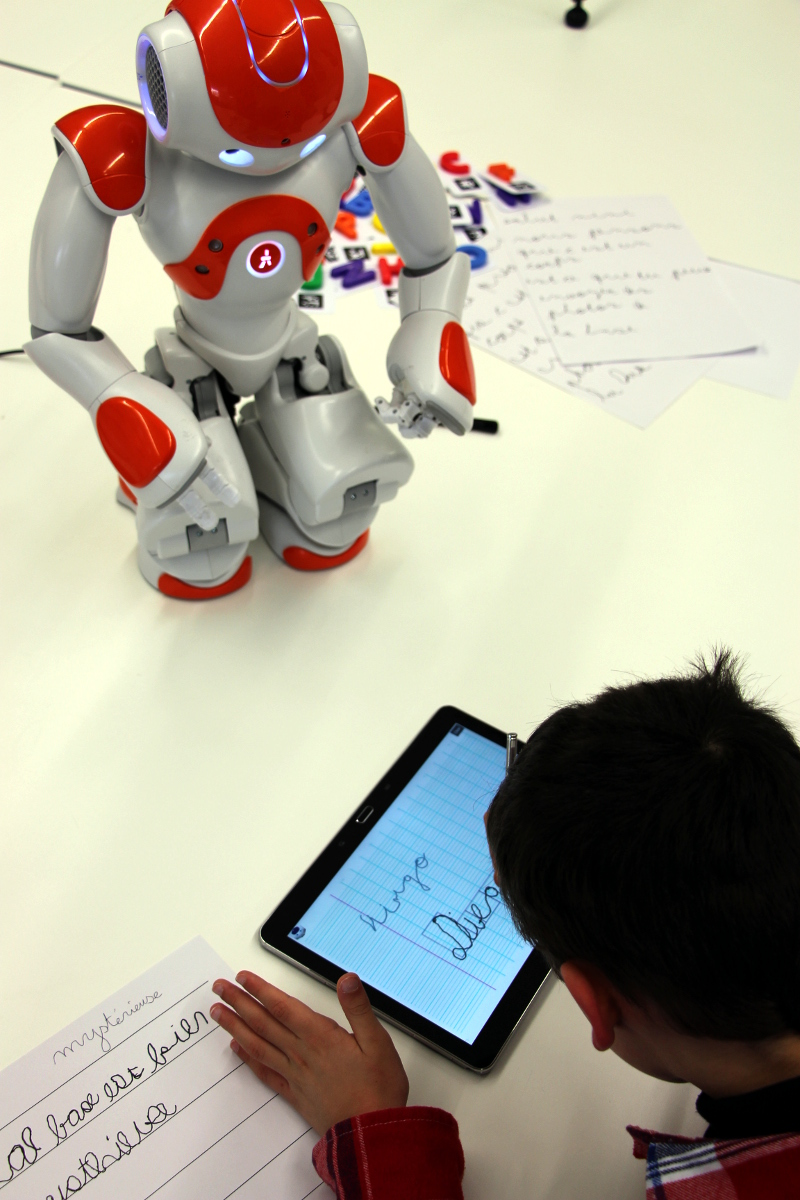
\includegraphics[width=0.5\linewidth]{diego}
    \caption{Diego working with Nao}
    \label{fig:diego}
\end{figure}


\subsubsection{Results}

\begin{figure}
    \centering
    \subfigure[Initial letter, generated by the robot]{
        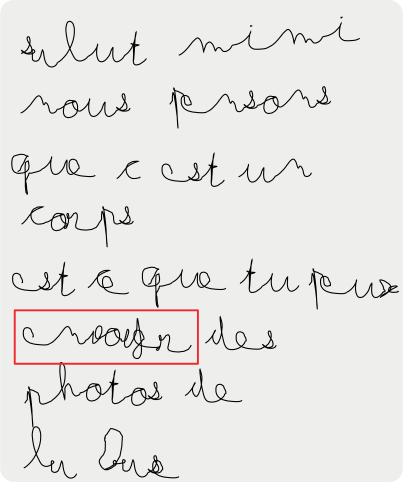
\includegraphics[height=6cm]{diego-initial-letter}
    }
    \subfigure[Final letter, after training with Diego]{
        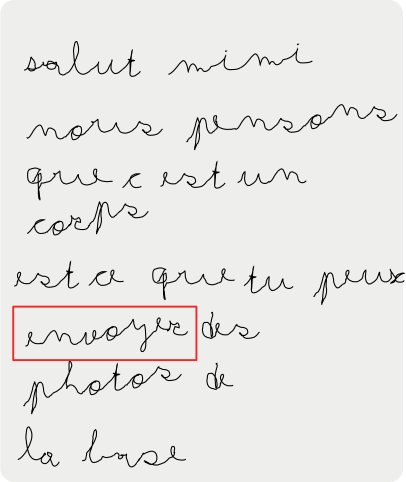
\includegraphics[height=6cm]{diego-final-letter}
    }

    \caption{\small Text generated by the robot, before and after training with
    the child. As an example, the red box emphasizes the changes on the word
    ``envoyer''.}
    \label{fig:stimuli}
\end{figure}


%%%%%%%%%%%%%%%%%%%%%%%%%%%%%%%%%%%%%%%%%%%%%%%%%%%%%%%%%%%%%%%%%%%%%%%%%%%%%%%%%%%
\subsection{Case Study 2: Henry}

\subsubsection{Context, Study Design}

\begin{figure}
    \centering
    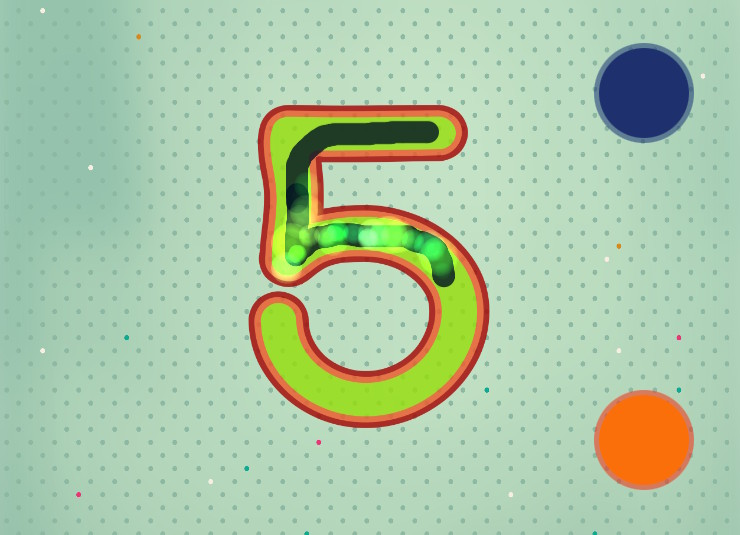
\includegraphics[width=0.9\linewidth]{abc-writer}
    \caption{Screenshot of the Android application developed to be used as
    pre-test and post-test: the child must follow with his finger the path of
the letter or number. We count the number of times the finger goes outside of
the red-bordered area.}
    \label{}
\end{figure}


\subsubsection{Results}

\begin{figure}
    \centering
    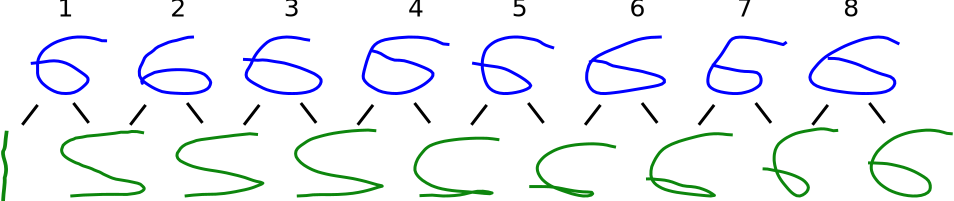
\includegraphics[width=0.9\linewidth]{learning_6_demos}
    \caption{Henry's demonstrations for the number ``6'' (top row) and
        corresponding shapes generated by the robot. After eight demomstrations,
        Henry decided that the robot's ``6'' was good enough, and went to
    another character: in that respect, he was the one leading the learning
process of the robot.}
    \label{henry_demos}
\end{figure}


\begin{figure}
    \centering
    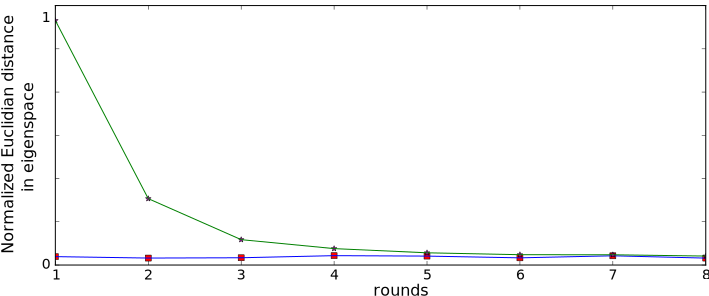
\includegraphics[width=0.9\linewidth]{learning_6_distances}
    \caption{Two metrics to assess the handwriting progresses: Euclidian
    distance in the Eigenspace of the number dataset (top figure) or in
cartesian space (bottom figure). Green lines represent the robot performance,
blue lines Henry's performance. The round IDs correspond to the demonstrations
pictured on Figure~\ref{henry_demos}.}
    \label{henry_distances}
\end{figure}



%%%%%%%%%%%%%%%%%%%%%%%%%%%%%%%%%%%%%%%%%%%%%%%%%%%%%%%%%%%%%%%%%%%%%%%%%%%%%%%%%%%
%%%%%%%%%%%%%%%%%%%%%%%%%%%%%%%%%%%%%%%%%%%%%%%%%%%%%%%%%%%%%%%%%%%%%%%%%%%%%%%%%%%
%%%%%%%%%%%%%%%%%%%%%%%%%%%%%%%%%%%%%%%%%%%%%%%%%%%%%%%%%%%%%%%%%%%%%%%%%%%%%%%%%%%
\section{Agency and Commitment}

However, we believe that the strongest impact of this work is for the
human-robot interaction community and relates to the very \emph{nature} of the
interaction fostered by this research. The work presented here investigates a
particular role for a robot in the education of handwriting: not only is the
robot actively performing the activity by drawing letters, but it does so in a
way that engages the child in a very specific social role. The child is the
teacher in this relationship and the robot is the learner: the child must engage
in a (meta-) cognitive relationship with the robot to try to understand why the
robot fails and how to help it best.  Here, the robot is more than just an
activity facilitator or orchestrator -- its physical presence and embodiment
induce agency and anthropomorphising, and cognitively engage the child into the
learning activity, which we predict will lead to higher learning efficacy.


%%%%%%%%%%%%%%%%%%%%%%%%%%%%%%%%%%%%%%%%%%%%%%%%%%%%%%%%%%%%%%%%%%%%%%%%%%%%%%%%%%%
%%%%%%%%%%%%%%%%%%%%%%%%%%%%%%%%%%%%%%%%%%%%%%%%%%%%%%%%%%%%%%%%%%%%%%%%%%%%%%%%%%%
\section*{Acknowledgments}

We would like to thank Deanna Hood for her key contribution to the project.
This research was partially supported by the Funda\c{c}\~{a}o para a Ci\^{e}ncia
e a Tecnologia (FCT) with reference UID/CEC/50021/2013, and by the Swiss
National Science Foundation through the National Centre of Competence in
Research Robotics.

\bibliographystyle{abbrv}
\bibliography{biblio}


\end{document}
